\section{Algorithmic Optimization in Architecture}
\label{sec: Methodology}

Through times, the architectural design paradigm has incrementally grown to develop the mechanisms to quickly (1) update a design, (2) generate the corresponding analytical model, and (3) automatically evaluate the design in an analytical tool. These mechanisms laid down the foundations for automated optimization processes. In fact, by extending the \ac{AD} and \ac{AA} approaches to include optimization mechanisms, we are able to apply automatic optimization processes that aim to improve (or even optimize) designs' performance. 

\Cref{fig:algorithmicoptimization} illustrates a possible approach for introducing automated optimization processes in the architectural worfklow. In this approach, we introduce an optimizer component that is responsible for searching the design space and generating new values for the design's parameters. These values are then communicated to the \ac{AD} tool, which generates the analytical models and evaluates them in the corresponding analytical tools. After being evaluated, the analytical tools communicate the evaluations' results to the \ac{AD} tool, which, in turn, forwards them to the optimizer. Based on these results, the optimizer generates another set of values for the design's parameters and this process is repeated until a stopping criterion (e.g., evaluations or time limit, solution's quality) is met. The communications between each component are encoded within the \ac{AD} tool, therefore incurring no additional efforts for the architect.

\begin{figure}[htbp]
	\centering
	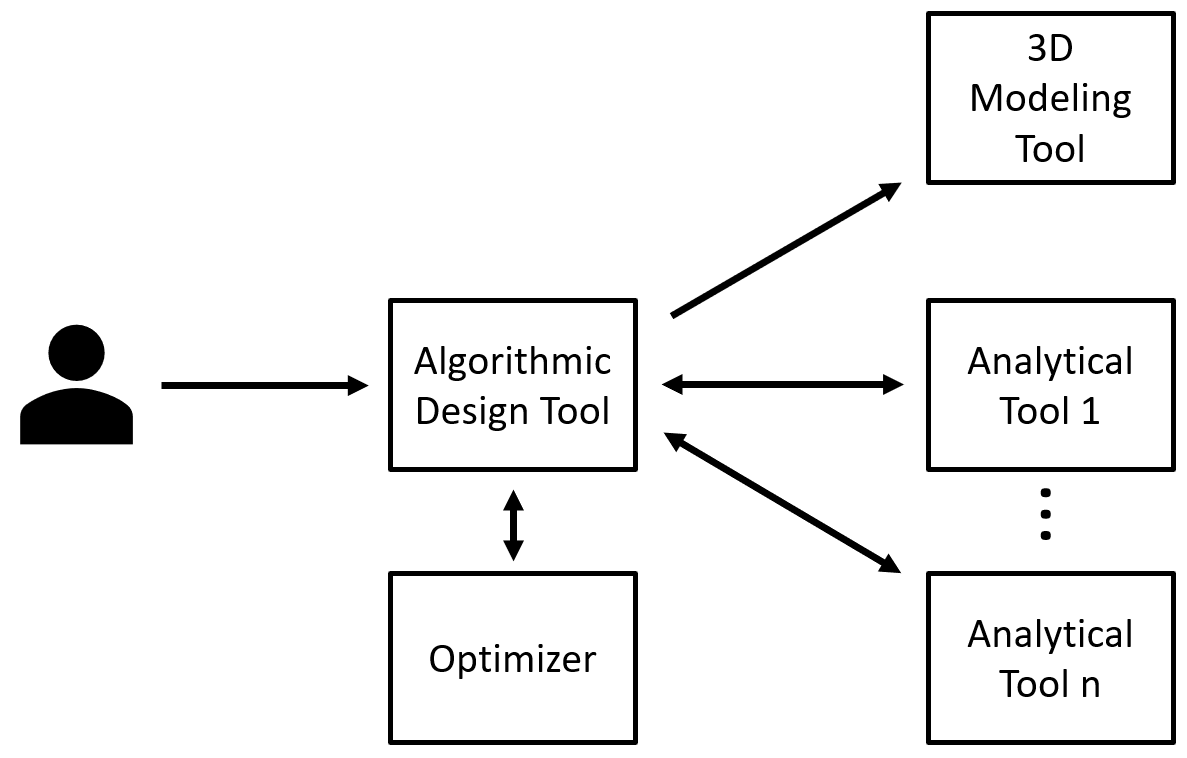
\includegraphics[width=\columnwidth]{../report/Images/Solution/algorithmic_optimization.png}
	\caption{Algorithmic Optimization workflow. In this workflow, the architect only interacts with an \ac{AD} tool to create the initial design, to specify the analysis tools, and to specify the optimization parameters.}
	\label{fig:algorithmicoptimization}
\end{figure}

In order to benefit from the \ac{AO} approach, we combine the optimization framework developed in this dissertation with an \ac{AD} tool to facilitate the resolution of a wide variety of \ac{BPO} problems. To this end, architects are required to: (1) create the \ac{AD} model reflecting their design's intents; (2) select the performance aspects to optimize and, thus, the analysis tools to be used (e.g., lighting, thermal, structural, costs), and, finally, (3) select, if necessary, the parameters of the optimization process (e.g., algorithm, algorithm's parameters).

One important aspect that results from this combination is that architects are able to use different optimization algorithms and, consequently, to opt for one that better suits their optimization problems. To circumvent the lack of knowledge regarding the most adequate choice of algorithms for each optimization problem, the optimization framework also provides automated testing mechanisms. These mechanisms enable the sequential execution of multiple optimization algorithms for a specified amount of evaluations, as well as each algorithm's performance measures. This feature is particularly important in the architectural context, as it promotes more informed decisions towards an adequate selection of optimization algorithms~\cite{Wortmann2016BBO,Hamdy2016}.

Due to the visual nature of architects and the generalized lack of confidence in optimization processes, the visualization of evaluated design solutions is of great importance, as it allows architects to explore and corroborate the optimization results. To this end, the optimization framework provides post-processing and visual mechanisms that, when combined with an \ac{AD} tool, allow the architect to click on the evaluated solutions and instantly visualize the corresponding design in a 3D modeling tool. 

These visual mechanisms also promote a better comprehension of the optimization process, as they allow architects to explore and visualize the results of the optimization, in real-time, to get a clearer perspective. Besides reasoning and creating logical patterns that allow them to explain the obtained results, architects can also learn more about their designs' behavior regarding different performance aspects and, potentially, about the optimization algorithm itself.

Finally, visualization and processing mechanisms can also be useful not only to detect errors or incoherences (e.g., in the optimization model) early in the optimization process, but also to reduce the overall optimization time, i.e.,  provide the architect with enough information to stop the optimization process sooner. For some problems, obtaining an optimum is not strictly necessary. Instead, a close to optimal or good solution suffices. Having a framework which interactively updates the information about the optimization process is particularly useful for those problems, since the user can explore and visualize the already evaluated candidate solutions and decide whether one of them suffices, even if it is not an optimum. 
